\documentclass[border=4pt]{standalone}
\usepackage{amsmath,amssymb,tikz}
\definecolor{figB}{RGB}{31,90,166}\definecolor{figR}{RGB}{176,48,48}\definecolor{figG}{RGB}{46,125,50}\definecolor{figO}{RGB}{214,120,20}
\begin{document}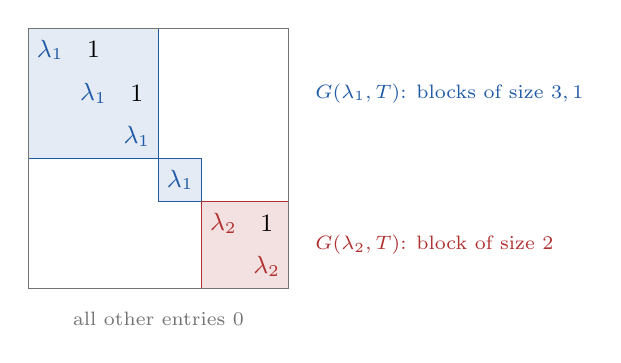
\begin{tikzpicture}[scale=0.55]
\fill[figB!12] (0,6) rectangle (3,3); \fill[figB!12] (3,3) rectangle (4,2); \fill[figR!15] (4,2) rectangle (6,0);
\draw[figB,thin] (0,6) rectangle (3,3); \draw[figB,thin] (3,3) rectangle (4,2); \draw[figR,thin] (4,2) rectangle (6,0);
\draw[black!55] (0,0) rectangle (6,6);
\foreach \i in {0,...,5} {\pgfmathsetmacro{\y}{5.5-\i}\pgfmathsetmacro{\x}{0.5+\i}
  \ifnum\i<4 \node[font=\small,figB] at (\x,\y) {$\lambda_1$};\else \node[font=\small,figR] at (\x,\y) {$\lambda_2$};\fi}
\node[font=\small] at (1.5,5.5) {$1$}; \node[font=\small] at (2.5,4.5) {$1$}; \node[font=\small] at (5.5,1.5) {$1$};
\node[font=\scriptsize,figB,anchor=west] at (6.4,4.5) {$G(\lambda_1,T)$: blocks of size $3,1$};
\node[font=\scriptsize,figR,anchor=west] at (6.4,1) {$G(\lambda_2,T)$: block of size $2$};
\node[font=\scriptsize,black!55] at (3,-0.7) {all other entries $0$};
\end{tikzpicture}\end{document}
